\documentclass[]{book}
\usepackage{lmodern}
\usepackage{amssymb,amsmath}
\usepackage{ifxetex,ifluatex}
\usepackage{fixltx2e} % provides \textsubscript
\ifnum 0\ifxetex 1\fi\ifluatex 1\fi=0 % if pdftex
  \usepackage[T1]{fontenc}
  \usepackage[utf8]{inputenc}
\else % if luatex or xelatex
  \ifxetex
    \usepackage{mathspec}
  \else
    \usepackage{fontspec}
  \fi
  \defaultfontfeatures{Ligatures=TeX,Scale=MatchLowercase}
\fi
% use upquote if available, for straight quotes in verbatim environments
\IfFileExists{upquote.sty}{\usepackage{upquote}}{}
% use microtype if available
\IfFileExists{microtype.sty}{%
\usepackage{microtype}
\UseMicrotypeSet[protrusion]{basicmath} % disable protrusion for tt fonts
}{}
\usepackage[margin=1in]{geometry}
\usepackage{hyperref}
\hypersetup{unicode=true,
            pdftitle={R for STATEC},
            pdfauthor={Bruno Rodrigues},
            pdfborder={0 0 0},
            breaklinks=true}
\urlstyle{same}  % don't use monospace font for urls
\usepackage{natbib}
\bibliographystyle{apalike}
\usepackage{color}
\usepackage{fancyvrb}
\newcommand{\VerbBar}{|}
\newcommand{\VERB}{\Verb[commandchars=\\\{\}]}
\DefineVerbatimEnvironment{Highlighting}{Verbatim}{commandchars=\\\{\}}
% Add ',fontsize=\small' for more characters per line
\usepackage{framed}
\definecolor{shadecolor}{RGB}{248,248,248}
\newenvironment{Shaded}{\begin{snugshade}}{\end{snugshade}}
\newcommand{\KeywordTok}[1]{\textcolor[rgb]{0.13,0.29,0.53}{\textbf{#1}}}
\newcommand{\DataTypeTok}[1]{\textcolor[rgb]{0.13,0.29,0.53}{#1}}
\newcommand{\DecValTok}[1]{\textcolor[rgb]{0.00,0.00,0.81}{#1}}
\newcommand{\BaseNTok}[1]{\textcolor[rgb]{0.00,0.00,0.81}{#1}}
\newcommand{\FloatTok}[1]{\textcolor[rgb]{0.00,0.00,0.81}{#1}}
\newcommand{\ConstantTok}[1]{\textcolor[rgb]{0.00,0.00,0.00}{#1}}
\newcommand{\CharTok}[1]{\textcolor[rgb]{0.31,0.60,0.02}{#1}}
\newcommand{\SpecialCharTok}[1]{\textcolor[rgb]{0.00,0.00,0.00}{#1}}
\newcommand{\StringTok}[1]{\textcolor[rgb]{0.31,0.60,0.02}{#1}}
\newcommand{\VerbatimStringTok}[1]{\textcolor[rgb]{0.31,0.60,0.02}{#1}}
\newcommand{\SpecialStringTok}[1]{\textcolor[rgb]{0.31,0.60,0.02}{#1}}
\newcommand{\ImportTok}[1]{#1}
\newcommand{\CommentTok}[1]{\textcolor[rgb]{0.56,0.35,0.01}{\textit{#1}}}
\newcommand{\DocumentationTok}[1]{\textcolor[rgb]{0.56,0.35,0.01}{\textbf{\textit{#1}}}}
\newcommand{\AnnotationTok}[1]{\textcolor[rgb]{0.56,0.35,0.01}{\textbf{\textit{#1}}}}
\newcommand{\CommentVarTok}[1]{\textcolor[rgb]{0.56,0.35,0.01}{\textbf{\textit{#1}}}}
\newcommand{\OtherTok}[1]{\textcolor[rgb]{0.56,0.35,0.01}{#1}}
\newcommand{\FunctionTok}[1]{\textcolor[rgb]{0.00,0.00,0.00}{#1}}
\newcommand{\VariableTok}[1]{\textcolor[rgb]{0.00,0.00,0.00}{#1}}
\newcommand{\ControlFlowTok}[1]{\textcolor[rgb]{0.13,0.29,0.53}{\textbf{#1}}}
\newcommand{\OperatorTok}[1]{\textcolor[rgb]{0.81,0.36,0.00}{\textbf{#1}}}
\newcommand{\BuiltInTok}[1]{#1}
\newcommand{\ExtensionTok}[1]{#1}
\newcommand{\PreprocessorTok}[1]{\textcolor[rgb]{0.56,0.35,0.01}{\textit{#1}}}
\newcommand{\AttributeTok}[1]{\textcolor[rgb]{0.77,0.63,0.00}{#1}}
\newcommand{\RegionMarkerTok}[1]{#1}
\newcommand{\InformationTok}[1]{\textcolor[rgb]{0.56,0.35,0.01}{\textbf{\textit{#1}}}}
\newcommand{\WarningTok}[1]{\textcolor[rgb]{0.56,0.35,0.01}{\textbf{\textit{#1}}}}
\newcommand{\AlertTok}[1]{\textcolor[rgb]{0.94,0.16,0.16}{#1}}
\newcommand{\ErrorTok}[1]{\textcolor[rgb]{0.64,0.00,0.00}{\textbf{#1}}}
\newcommand{\NormalTok}[1]{#1}
\usepackage{longtable,booktabs}
\usepackage{graphicx,grffile}
\makeatletter
\def\maxwidth{\ifdim\Gin@nat@width>\linewidth\linewidth\else\Gin@nat@width\fi}
\def\maxheight{\ifdim\Gin@nat@height>\textheight\textheight\else\Gin@nat@height\fi}
\makeatother
% Scale images if necessary, so that they will not overflow the page
% margins by default, and it is still possible to overwrite the defaults
% using explicit options in \includegraphics[width, height, ...]{}
\setkeys{Gin}{width=\maxwidth,height=\maxheight,keepaspectratio}
\IfFileExists{parskip.sty}{%
\usepackage{parskip}
}{% else
\setlength{\parindent}{0pt}
\setlength{\parskip}{6pt plus 2pt minus 1pt}
}
\setlength{\emergencystretch}{3em}  % prevent overfull lines
\providecommand{\tightlist}{%
  \setlength{\itemsep}{0pt}\setlength{\parskip}{0pt}}
\setcounter{secnumdepth}{5}
% Redefines (sub)paragraphs to behave more like sections
\ifx\paragraph\undefined\else
\let\oldparagraph\paragraph
\renewcommand{\paragraph}[1]{\oldparagraph{#1}\mbox{}}
\fi
\ifx\subparagraph\undefined\else
\let\oldsubparagraph\subparagraph
\renewcommand{\subparagraph}[1]{\oldsubparagraph{#1}\mbox{}}
\fi

%%% Use protect on footnotes to avoid problems with footnotes in titles
\let\rmarkdownfootnote\footnote%
\def\footnote{\protect\rmarkdownfootnote}

%%% Change title format to be more compact
\usepackage{titling}

% Create subtitle command for use in maketitle
\newcommand{\subtitle}[1]{
  \posttitle{
    \begin{center}\large#1\end{center}
    }
}

\setlength{\droptitle}{-2em}
  \title{R for STATEC}
  \pretitle{\vspace{\droptitle}\centering\huge}
  \posttitle{\par}
  \author{Bruno Rodrigues}
  \preauthor{\centering\large\emph}
  \postauthor{\par}
  \predate{\centering\large\emph}
  \postdate{\par}
  \date{2017-10-10}

\usepackage{booktabs}

\usepackage{amsthm}
\newtheorem{theorem}{Theorem}[chapter]
\newtheorem{lemma}{Lemma}[chapter]
\theoremstyle{definition}
\newtheorem{definition}{Definition}[chapter]
\newtheorem{corollary}{Corollary}[chapter]
\newtheorem{proposition}{Proposition}[chapter]
\theoremstyle{definition}
\newtheorem{example}{Example}[chapter]
\theoremstyle{definition}
\newtheorem{exercise}{Exercise}[chapter]
\theoremstyle{remark}
\newtheorem*{remark}{Remark}
\newtheorem*{solution}{Solution}
\begin{document}
\maketitle

{
\setcounter{tocdepth}{1}
\tableofcontents
}
\chapter{What is R?}\label{what-is-r}

Read R's official answer to this question
\href{https://cran.r-project.org/doc/FAQ/R-FAQ.html\#What-is-R_003f}{here}.
To make it short: R is multi-paradigm (procedural, imperative,
object-oriented and functional) \footnote{In this book we are going to
  focus on R's functional programming capabilities} programming language
that focuses on applications in \emph{statistics}. By \emph{statistics}
I mean any field that uses statistics such as official statistics,
economics, finance, data science, etc.

\section{Prerequisites}\label{prerequisites}

R and Rstudio are the two main pieces of software that we are going to
use. Both are already installed on your desktop computer. R is the
programming language and Rstudio is a modern IDE for it. R and Rstudio
are both open source: this means that the source code is freely
available on the internet and contributions by anyone are welcome and
integrated; provided they are meaningful and useful.

If you wish to install R and Rstudio at home to follow the examples in
this book you can do it as both pieces of software are available free of
charge (for firms paid options for Rstudio exist). Installation is
simple, but operating system dependent. To download and install R for
Windows, follow
\href{https://cloud.r-project.org/bin/windows/base/}{this link}. For
macOS, follow \href{https://cloud.r-project.org/bin/macosx/}{this one}.
If you run a GNU+Linux distribution, you can install R using the
system's package manager. On Ubuntu, install \texttt{r-base}.

For Rstudio, look for your operating system
\href{https://www.rstudio.com/products/rstudio/download/\#download}{here}.

\section{What are packages?}\label{what-are-packages}

There is one more step; we are going to install some packages. Packages
are additional pieces of code that can be installed from within R with
the following function: \texttt{install.packages()}. These packages
extend R's capabilities significantly, and are probably one of the main
reasons R is so popular. As of October 2017, R has over 11000 packages.

To install the packages we need, first open Rstudio and then copy and
paste this line in the console:

\begin{Shaded}
\begin{Highlighting}[]
\KeywordTok{install.packages}\NormalTok{(}\KeywordTok{c}\NormalTok{(}\StringTok{"tidyverse"}\NormalTok{, }\StringTok{"checkpoint"}\NormalTok{, }\StringTok{"eurostat"}\NormalTok{, }\StringTok{"ggthemes"}\NormalTok{, }\StringTok{"janitor"}\NormalTok{, }\StringTok{"openxlsx"}\NormalTok{))}
\end{Highlighting}
\end{Shaded}

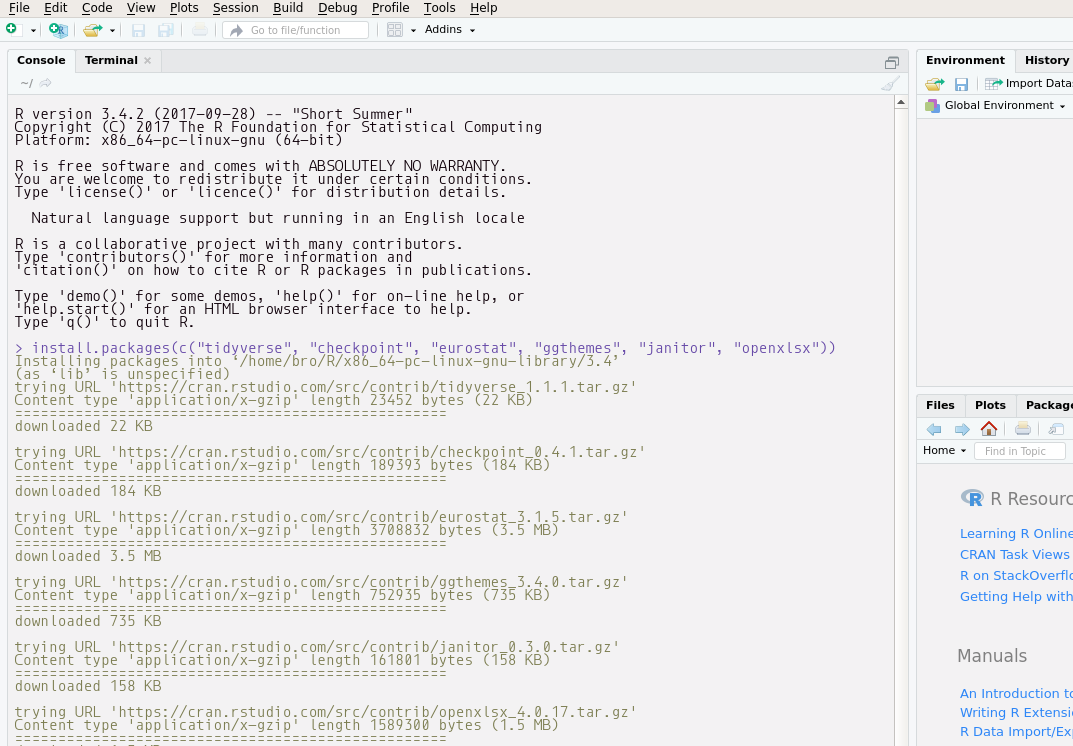
\includegraphics[width=14.9in]{pics/install_packages}

or go to the \textbf{Packages} pane and then click on \emph{Install}:

\includegraphics{pics/rstudio_install_packages.gif}

\chapter{Getting to know Rstudio}\label{getting-to-know-rstudio}

Rstudio is a modern IDE that makes writing R code easier. In this
chapter, we will learn about some of Rstudio's most useful features.

\section{Panes}\label{panes}

Rstudio is divided into different panes. Each pane has a specific
function. The gif below shows some of these panes:

\includegraphics{pics/rstudio_panes.gif}

Take some time to look around what each pane shows you. Some panes are
empty; for example the \emph{Plots} pane or the \emph{Viewer} pane.
\emph{Plots} shows you the plots you make. You can browse the plots and
save them. We will see this in more detail in a later chapter.
\emph{Viewer} shows you previews of documents that you generate with R.
More on this later.

Look at the gif below:

\includegraphics{pics/rstudio_new_script.gif}

In this gif, we see the user creating a new R script. R scripts are
simple text files that hold R code. Think of \texttt{.do} files in STATA
or \texttt{.c} files for C. R scripts have the extension \texttt{.r} or
\texttt{.R}.

\section{Options}\label{options}

It is also possible to customize Rstudio's look and feel:

\includegraphics{pics/rstudio_options.gif}

Take some time to go through the options.

\section{Keyboard shortcuts}\label{keyboard-shortcuts}

It is a good idea to familiarize yourself with at least some keyboard
shortcuts. This is more convenient than having to move the mouse around:

\includegraphics{pics/rstudio_shortcuts.gif}

If there is only one keyboard shortcut you need to know, it's
\texttt{Ctrl-Enter} that executes a line of code from your script.

\section{Projects}\label{projects}

\chapter{Literature}\label{literature}

Here is a review of existing methods.

\chapter{Methods}\label{methods}

We describe our methods in this chapter.

\chapter{Applications}\label{applications}

Some \emph{significant} applications are demonstrated in this chapter.

\section{Example one}\label{example-one}

\section{Example two}\label{example-two}

\chapter{Final Words}\label{final-words}

We have finished a nice book.

\bibliography{packages.bib,book.bib}


\end{document}
